% \documentclass[10pt,draft]{beamer}
\documentclass[10pt]{beamer}

\usetheme{metropolis}
\usepackage{appendixnumberbeamer}
\usepackage{tikz}
\usetikzlibrary{decorations.pathreplacing}
\usepackage{caption}
\usepackage{graphicx}
\usepackage{multirow}
\usepackage{listings}
\usepackage{booktabs}
\usepackage{minted}
\usepackage{algorithm}
\usepackage[noend]{algpseudocode}
\pgfdeclarelayer{bg}    % declare background layer
\pgfsetlayers{bg,main}  % set the order of the layers (main is the standard layer)
\usepackage{pgfplots}
\usepgfplotslibrary{dateplot}

\usepackage{booktabs}
\usepackage[scale=2]{ccicons}
\usepackage{adjustbox}

\usepackage{xspace}
\newcommand{\themename}{\textbf{\textsc{metropolis}}\xspace}
\usepackage{natbib}
\usepackage{color}
\newcommand{\todo}[1]{\textbf{\textcolor{red}{#1}}}
\def\stackplotStart{2013-12-21} 
\def\stackplotEnd{2018-12-19} 

\title{A Deep Dive into Bitcoin Mining Pools}
\subtitle{An Empirical Analysis of Mining Shares}

\author[shortname]{\textbf{Matteo Romiti} \inst{1}\and
Aljosha Judmayer \inst{2} \\ \and
Alexei Zamyatin \inst{2}\textsuperscript{,} \inst{3} \and
Bernhard Haslhofer \inst{1}}


\institute[shortinst]{\inst{1} Austrian Institute of Technology \and
\inst{2} SBA Research \and \inst{3} Imperial College London}

% \date{\today}

\begin{document}

\maketitle

\begin{frame}[fragile]{Introduction}
    \textbf{Why do we care about miners?} \pause
    \begin{itemize}
        \item Miners decide which transactions to include in a block \pause
        \item Miners decide which blocks to include in the chain \pause
        \item Miners are rewarded with new coins and transaction fees \pause
        \item Miners secure the network (Proof-of-Work algorithm) \pause
        \item Miners can attack the network (e.g., double-spend) 
    \end{itemize}
\end{frame}

\begin{frame}[fragile]{Introduction}
    \textbf{What about Mining Pools?} \pause
    \begin{itemize}
        \item Solo mining is not profitable anymore \pause
        \item Miners join pools for steadier revenues \pause
        \item Miners can join multiple pools (Cross-Pool Mining) \pause
        \item Pools compete to create blocks and claim the rewards \pause
        \item Pool managers coordinate work and rewards among members
    \end{itemize}
\end{frame}

\begin{frame}[fragile]{Introduction}
    \textbf{Research Questions} \pause 
    \begin{enumerate}
        \item How did the mining centralization evolve over time? \pause
        \item How can we detect payments to pool members? \pause
        \item How decentralized is a mining pool? What do we know about pool members?
        % \item How decentralized is a mining pool? Who are the pool members? What’s their behavior?
    \end{enumerate}
\end{frame}

\section{Background} 
\begin{frame}[fragile]{Background | Coinbase Flow}
    \begin{figure}
        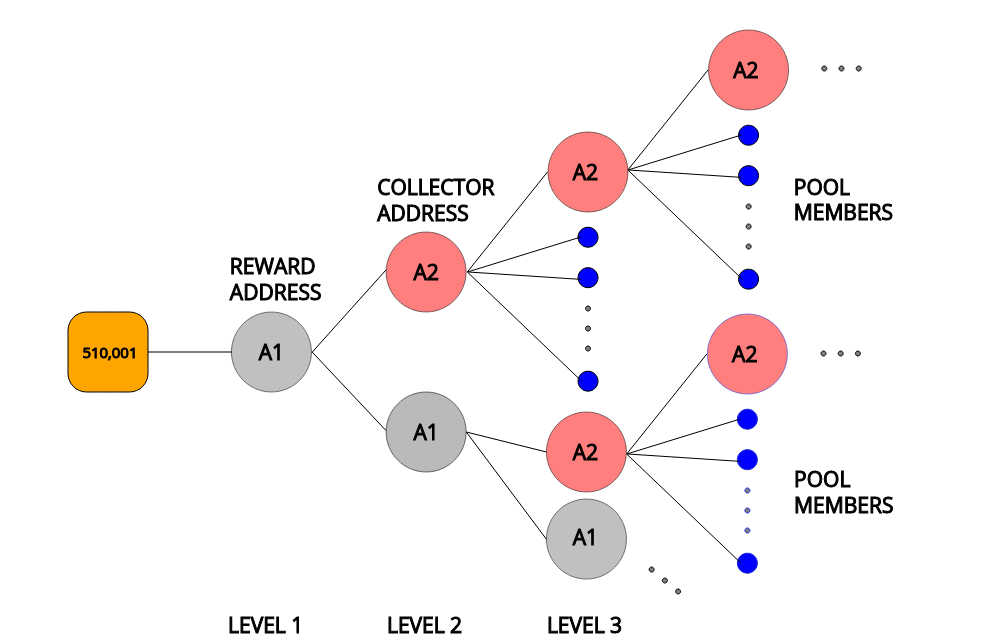
\includegraphics[width=.8\textwidth]{images/flow_example.png}
        \\Example of a coinbase flow
    \end{figure}
\end{frame}

\begin{frame}[fragile]{Background | Coinbase Flow}
    \begin{figure}
        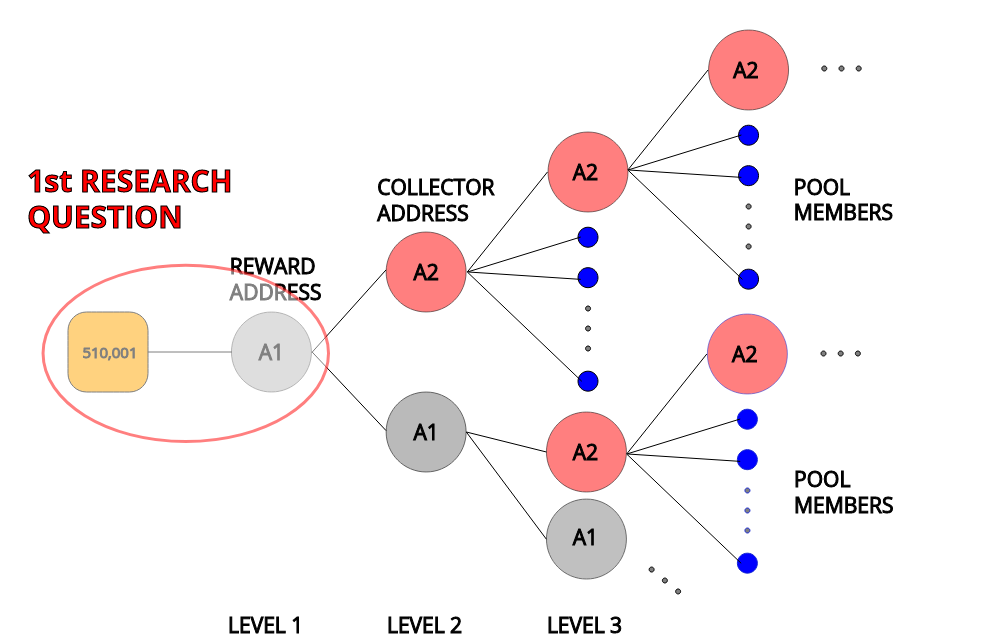
\includegraphics[width=.8\textwidth]{images/1rq.png}
        \\Example of a coinbase flow
    \end{figure}
\end{frame}

\begin{frame}[fragile]{Background | Coinbase Flow}
    \begin{figure}
        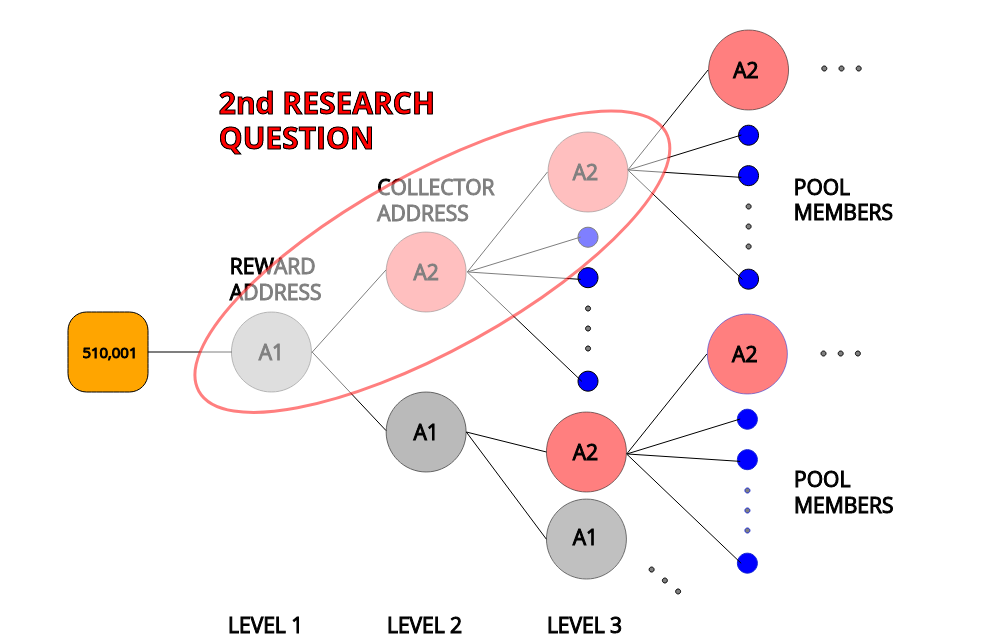
\includegraphics[width=.8\textwidth]{images/2rq.png}
        \\Example of a coinbase flow
    \end{figure}
\end{frame}

\begin{frame}[fragile]{Background | Coinbase Flow}
    \begin{figure}
        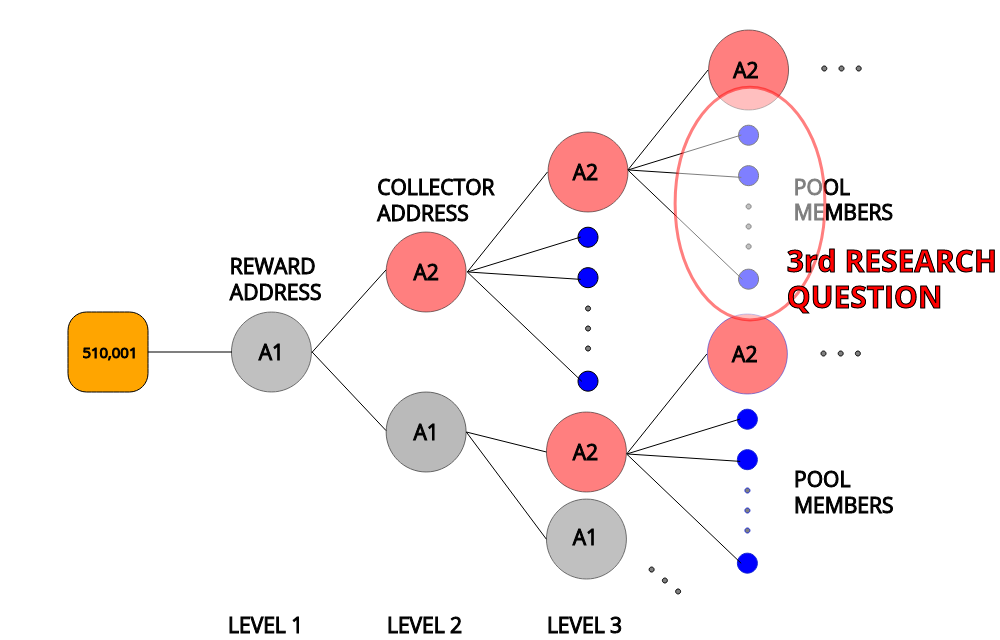
\includegraphics[width=.8\textwidth]{images/3rq.png}
        \\Example of a coinbase flow
    \end{figure}
\end{frame}

\begin{frame}[fragile]{Background | Multiple-Input Clustering Heuristic}
    \begin{figure}
        \centering
        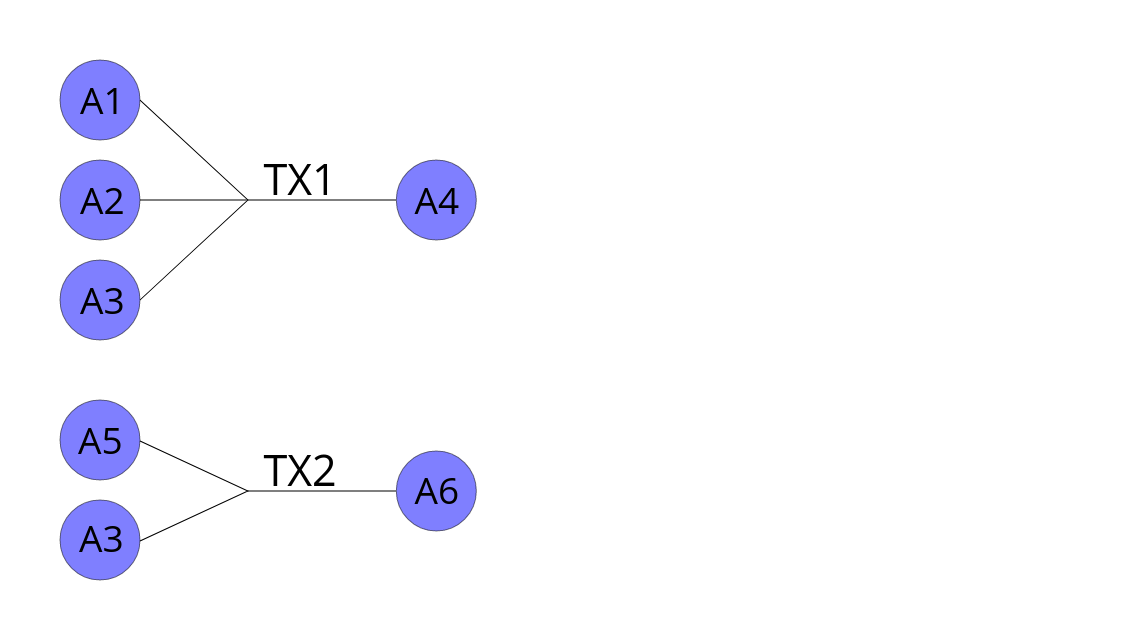
\includegraphics[width=0.9\textwidth]{images/clustering1.png}
        \\Multiple-input clustering heuristic
    \end{figure}
\end{frame}

\begin{frame}[fragile]{Background | Multiple-Input Clustering Heuristic}
    \begin{figure}
        \centering
        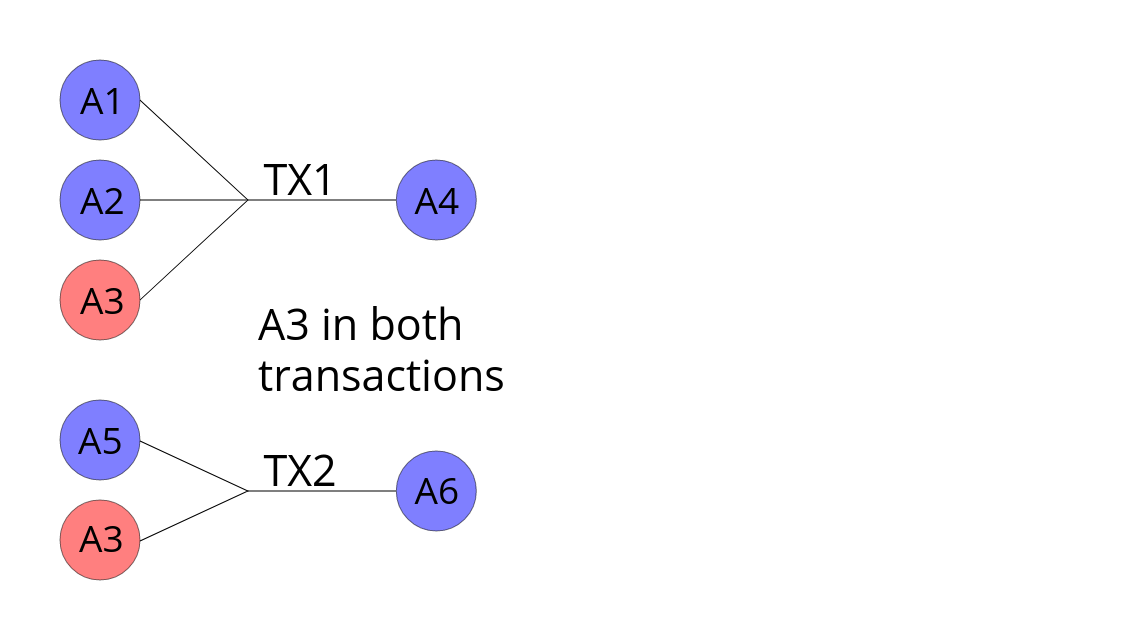
\includegraphics[width=0.9\textwidth]{images/clustering2.png}
        \\Multiple-input clustering heuristic
    \end{figure}
\end{frame}

\begin{frame}[fragile]{Background | Multiple-Input Clustering Heuristic}
    \begin{figure}
        \centering
        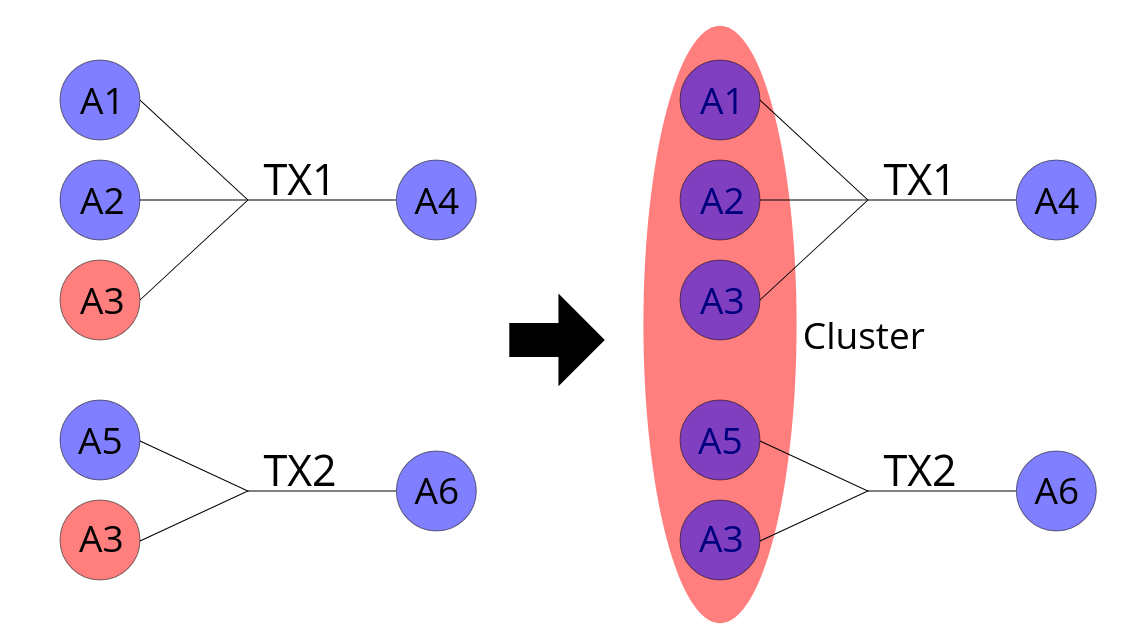
\includegraphics[width=0.9\textwidth]{images/clustering3.png}
        \\Multiple-input clustering heuristic
    \end{figure}
\end{frame}

\begin{frame}[fragile]{Background | Multiple-Input Clustering Heuristic}
    \begin{figure}
        \centering
        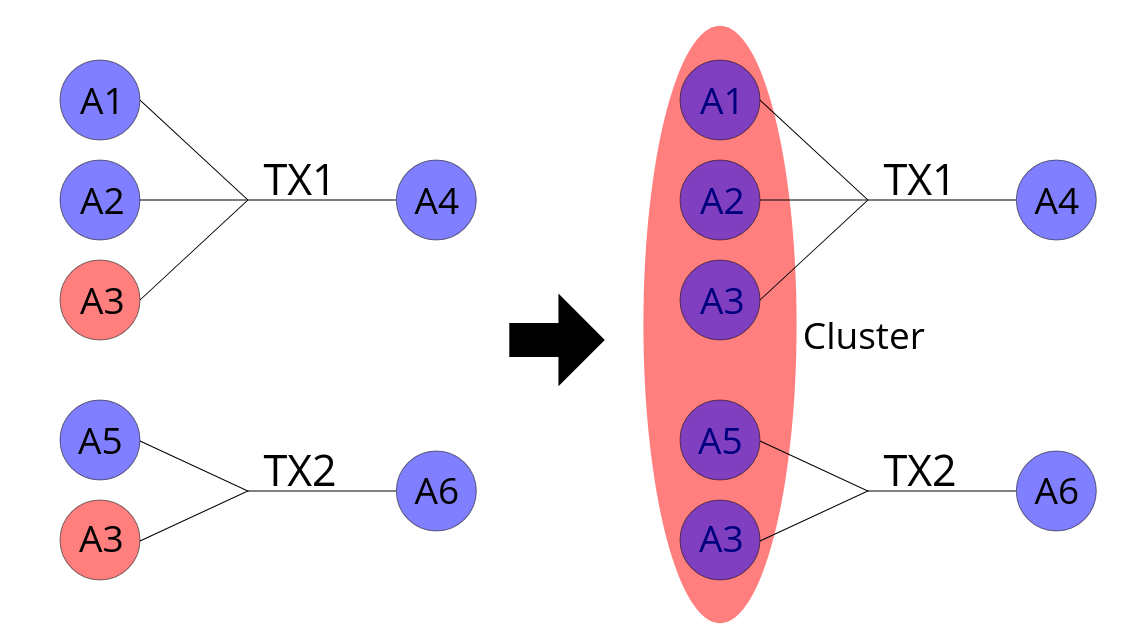
\includegraphics[width=0.9\textwidth]{images/clustering3.png}
    \end{figure}
    \begin{figure}
        \centering
        \def\svgwidth{\columnwidth}
        \input{images/graphsense.pdf_tex}
    \end{figure}
\end{frame}

\section{How did the mining centralization evolve?}
\begin{frame}[fragile]{Block Attribution | Data Sources}
    We combined different publicly-available data sources:
    \begin{itemize}
        \item Blocktrail API (till block 514239, March 2018)
        \item Blockchain.info Github repository
        \item BTC.com Github repository
        \item GraphSense
        \item Coinbase markers manually retrieved
    \end{itemize}
\end{frame}

\begin{frame}[fragile]{Block Attribution | Conflicts}
    \setlength{\tabcolsep}{2pt}
    \begin{table}
        684 attribution conflicts out of 556400 blocks (0.0012\%)
        \scalebox{.9}{
            \begin{tabular}{@{}llr@{}}
            \toprule
            Miner 1       & Miner 2         & \#Conflicts \\
            \midrule
            BTC.TOP       & CANOE           & 338                 \\
            Bixin         & TangPool        & 142                 \\
            BTC.com       & Waterhole       & 113                 \\
            BTC.TOP       & WAYI.CN         & 81                  \\
            ViaBTC        & Okminer         & 5                   \\
            Yourbtc       & OzCoin          & 3                   \\
            BitcoinRussia & Bitcoin-Ukraine & 1                   \\
            F2Pool        & BTCC Pool       & 1                   \\
            \bottomrule
            \end{tabular}
        }
    \end{table}
\end{frame}

\begin{frame}[fragile]{Block Attribution | Mining Pools' Shares}
        \vspace*{-0.77cm}
        \begin{figure}
            \hspace*{-1.7cm}
            \includegraphics[width=1.23\textwidth]{images/stackplot_periodLen_2016secs_end_554399_numPeriods_138_threshold_4_groupBy_miner.pdf}
            \\Evolution of mining pools' shares (\stackplotStart~to \stackplotEnd)
        \end{figure}
\end{frame}

\begin{frame}[fragile]{Block Attribution | Mining Pools' Shares}
     \vspace*{-0.77cm}
     \begin{tikzpicture}
            \node (image) at (current page.center) {
                \hspace*{-1.85cm}
                \includegraphics[width=1.23\textwidth]{images/stackplot_periodLen_2016secs_end_554399_numPeriods_138_threshold_4_groupBy_miner.pdf}
                };
            \begin{scope}[x={(image.south east)},y={(image.north west)}]
             \node[font=\large,inner sep=4pt,align=center] (Bitmain2) at (0.9,0.2) 
                {Bitmain};
             \draw[ultra thick,red,-stealth] (Bitmain2) -- (0.7,0.18);
             \draw[ultra thick,red,-stealth] (Bitmain2) -- (0.7,0.3);
             \draw[ultra thick,red,-stealth] (Bitmain2) -- (0.7,0.4);
            \end{scope}
    \end{tikzpicture}
\end{frame}

\begin{frame}[fragile]{Block Attribution | Mining Pools' Shares}
     \vspace*{-0.77cm}
     \begin{tikzpicture}
            \node (image) at (current page.center) {
                \hspace*{-1.85cm}
                \includegraphics[width=1.23\textwidth]{images/stackplot_periodLen_2016secs_end_554399_numPeriods_138_threshold_4_groupBy_miner.pdf}
                };
            \begin{scope}[x={(image.south east)},y={(image.north west)}]
             \node[font=\large,inner sep=4pt,align=center] (China) at (0.89,0.315) 
                {China};
             \draw[ultra thick,red,-stealth] (China) -- (0.7,0.18);
             \draw[ultra thick,red,-stealth] (China) -- (0.7,0.3);
             \draw[ultra thick,red,-stealth] (China) -- (0.7,0.4);
             \draw[ultra thick,red,-stealth] (China) -- (0.7,0.47);
             \draw[ultra thick,red,-stealth] (China) -- (0.77,0.54);
            \end{scope}
    \end{tikzpicture}
\end{frame}

\section{How can we detect payments to pool members?}
\begin{frame}[fragile]{Payout Patterns | Data Sources}
    \begin{itemize}
        \item Coinbase flows from Blockchain.info API
        \begin{figure}
            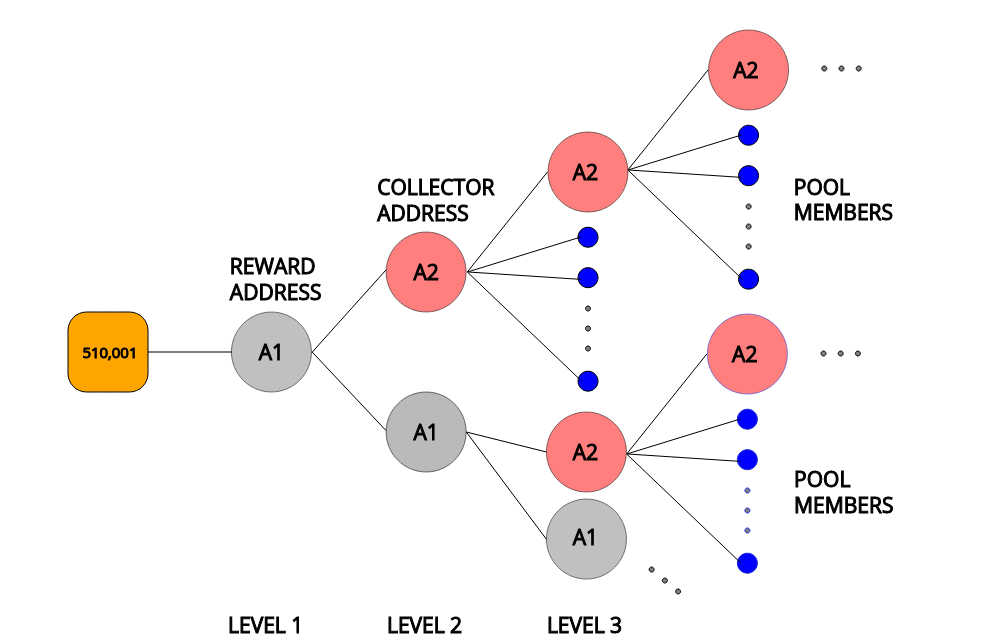
\includegraphics[width=.4\textwidth]{images/flow_example.png}
        \end{figure}
        \pause

        \item Focus on BTC.com, AntPool and ViaBTC
        \begin{figure}
            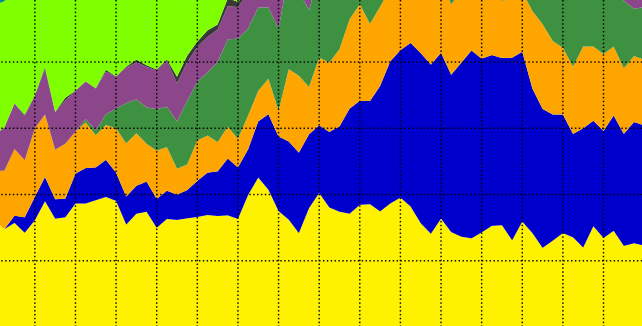
\includegraphics[width=.35\textwidth]{images/selected_pools.png}
        \end{figure} 

    \end{itemize}
\end{frame}

\begin{frame}[fragile]{Payout Patterns | BTC.com}
    \begin{figure}
        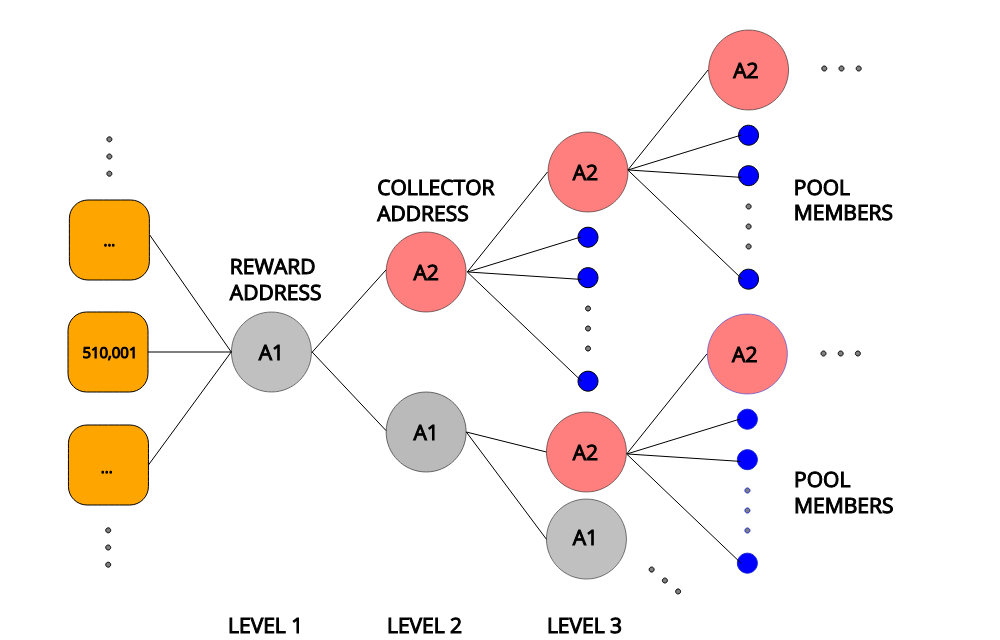
\includegraphics[width=.8\textwidth]{images/flow_BTCcom_example1.png}
        \\BTC.com payout pattern between block 510,000 and 514,032
    \end{figure}
\end{frame}

\begin{frame}[fragile]{Payout Patterns | AntPool}
    \begin{figure}
        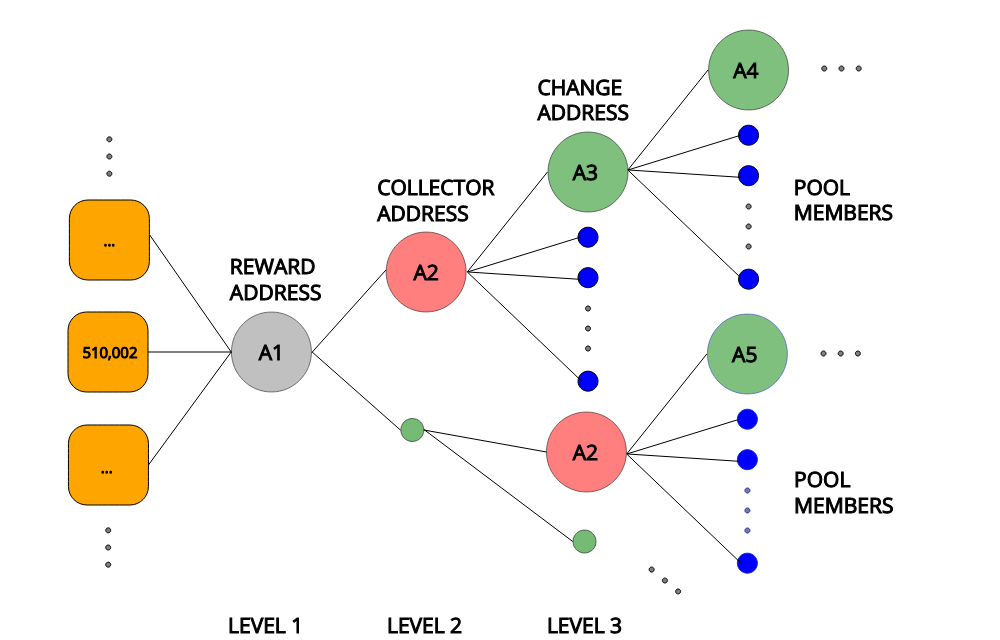
\includegraphics[width=.8\textwidth]{images/flow_AntPool_example1.png}
        \\AntPool payout pattern between block 510,000 and 514,032
    \end{figure}
\end{frame}

\begin{frame}[fragile]{Payout Patterns | ViaBTC}
    \begin{figure}
        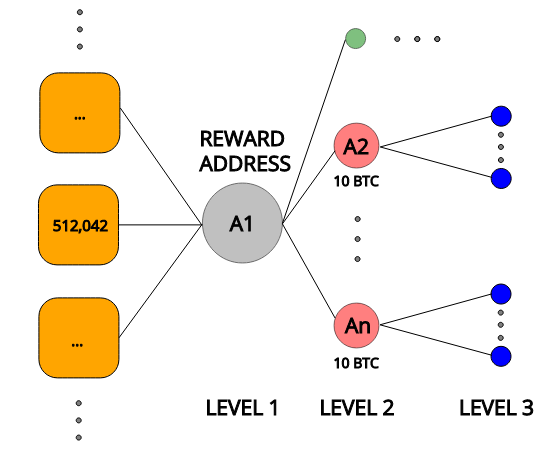
\includegraphics[width=.5\textwidth]{images/flow_ViaBTC_example2.png}
        \\ViaBTC payout pattern observed between block 510,000 and 514,032
    \end{figure}
\end{frame}

\begin{frame}[fragile]{Payout Patterns | Results}
    \setlength{\tabcolsep}{2pt}
    \begin{table}
        \centering
        Statistics of data retrieved between block 510,000 and 514,032
        \scalebox{0.95}{
            \begin{tabular}{@{}lrrrr@{}}
                \toprule
                Pool & 
\multicolumn{1}{c}{\begin{tabular}[c]{@{}c@{}}Mined\\ Blocks\end{tabular}} &
\multicolumn{1}{c}{\begin{tabular}[c]{@{}c@{}}Txs\\ Found\end{tabular}} &
\multicolumn{1}{c}{\begin{tabular}[c]{@{}c@{}}BTC\\ Coverage\end{tabular}} &
\multicolumn{1}{c}{\begin{tabular}[c]{@{}c@{}}Address\\ Reuse\\ Index\end{tabular}}  \\
                \midrule
                BTC.com     &1,020  &225    &92\%   &9.8 \\
                AntPool     &617    &408    &30\%   &1.4 \\
                ViaBTC      &457    &104    &75\%   &7.0 \\
                \bottomrule
            \end{tabular}   
        }
    \end{table}
\end{frame}

\section{How decentralized is a mining pool? What do we know about pool members?}
\begin{frame}[fragile]{Pools Members | Data Sources}

    \begin{itemize}
        \item Payout transactions (BTC.com, AntPool and ViaBTC)
        \begin{figure}
            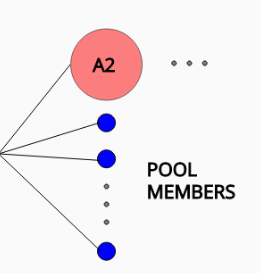
\includegraphics[width=.15\textwidth]{images/pool_members.png}
        \end{figure}
        \item GraphSense (Clustering and Tags)
        \begin{figure}
            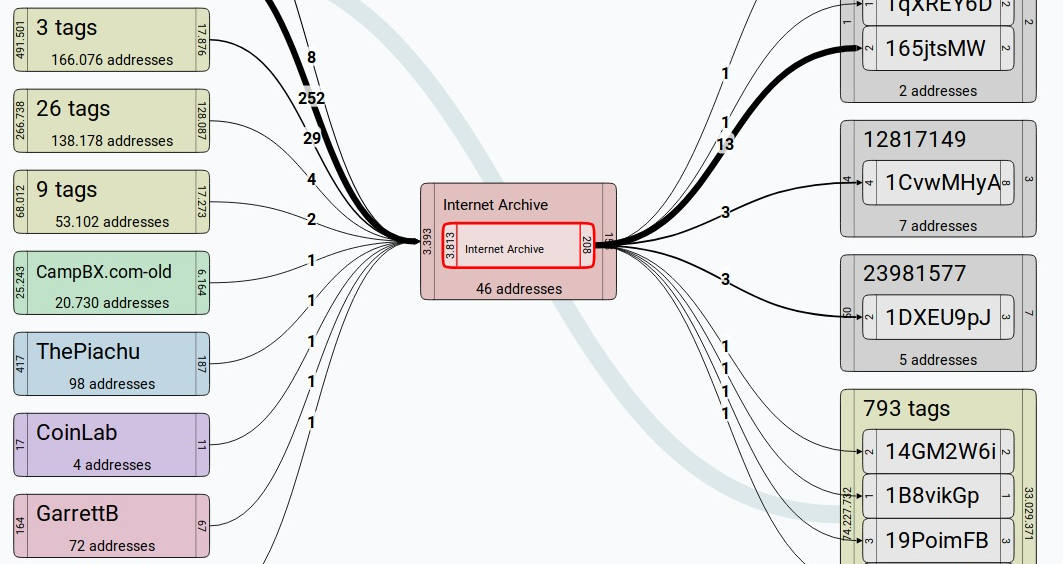
\includegraphics[width=.5\textwidth]{images/graphsense_graph.png}
        \end{figure}

    \end{itemize}


\end{frame}

\begin{frame}[fragile]{Pools Members | Pool Centralization}
    \begin{figure}
        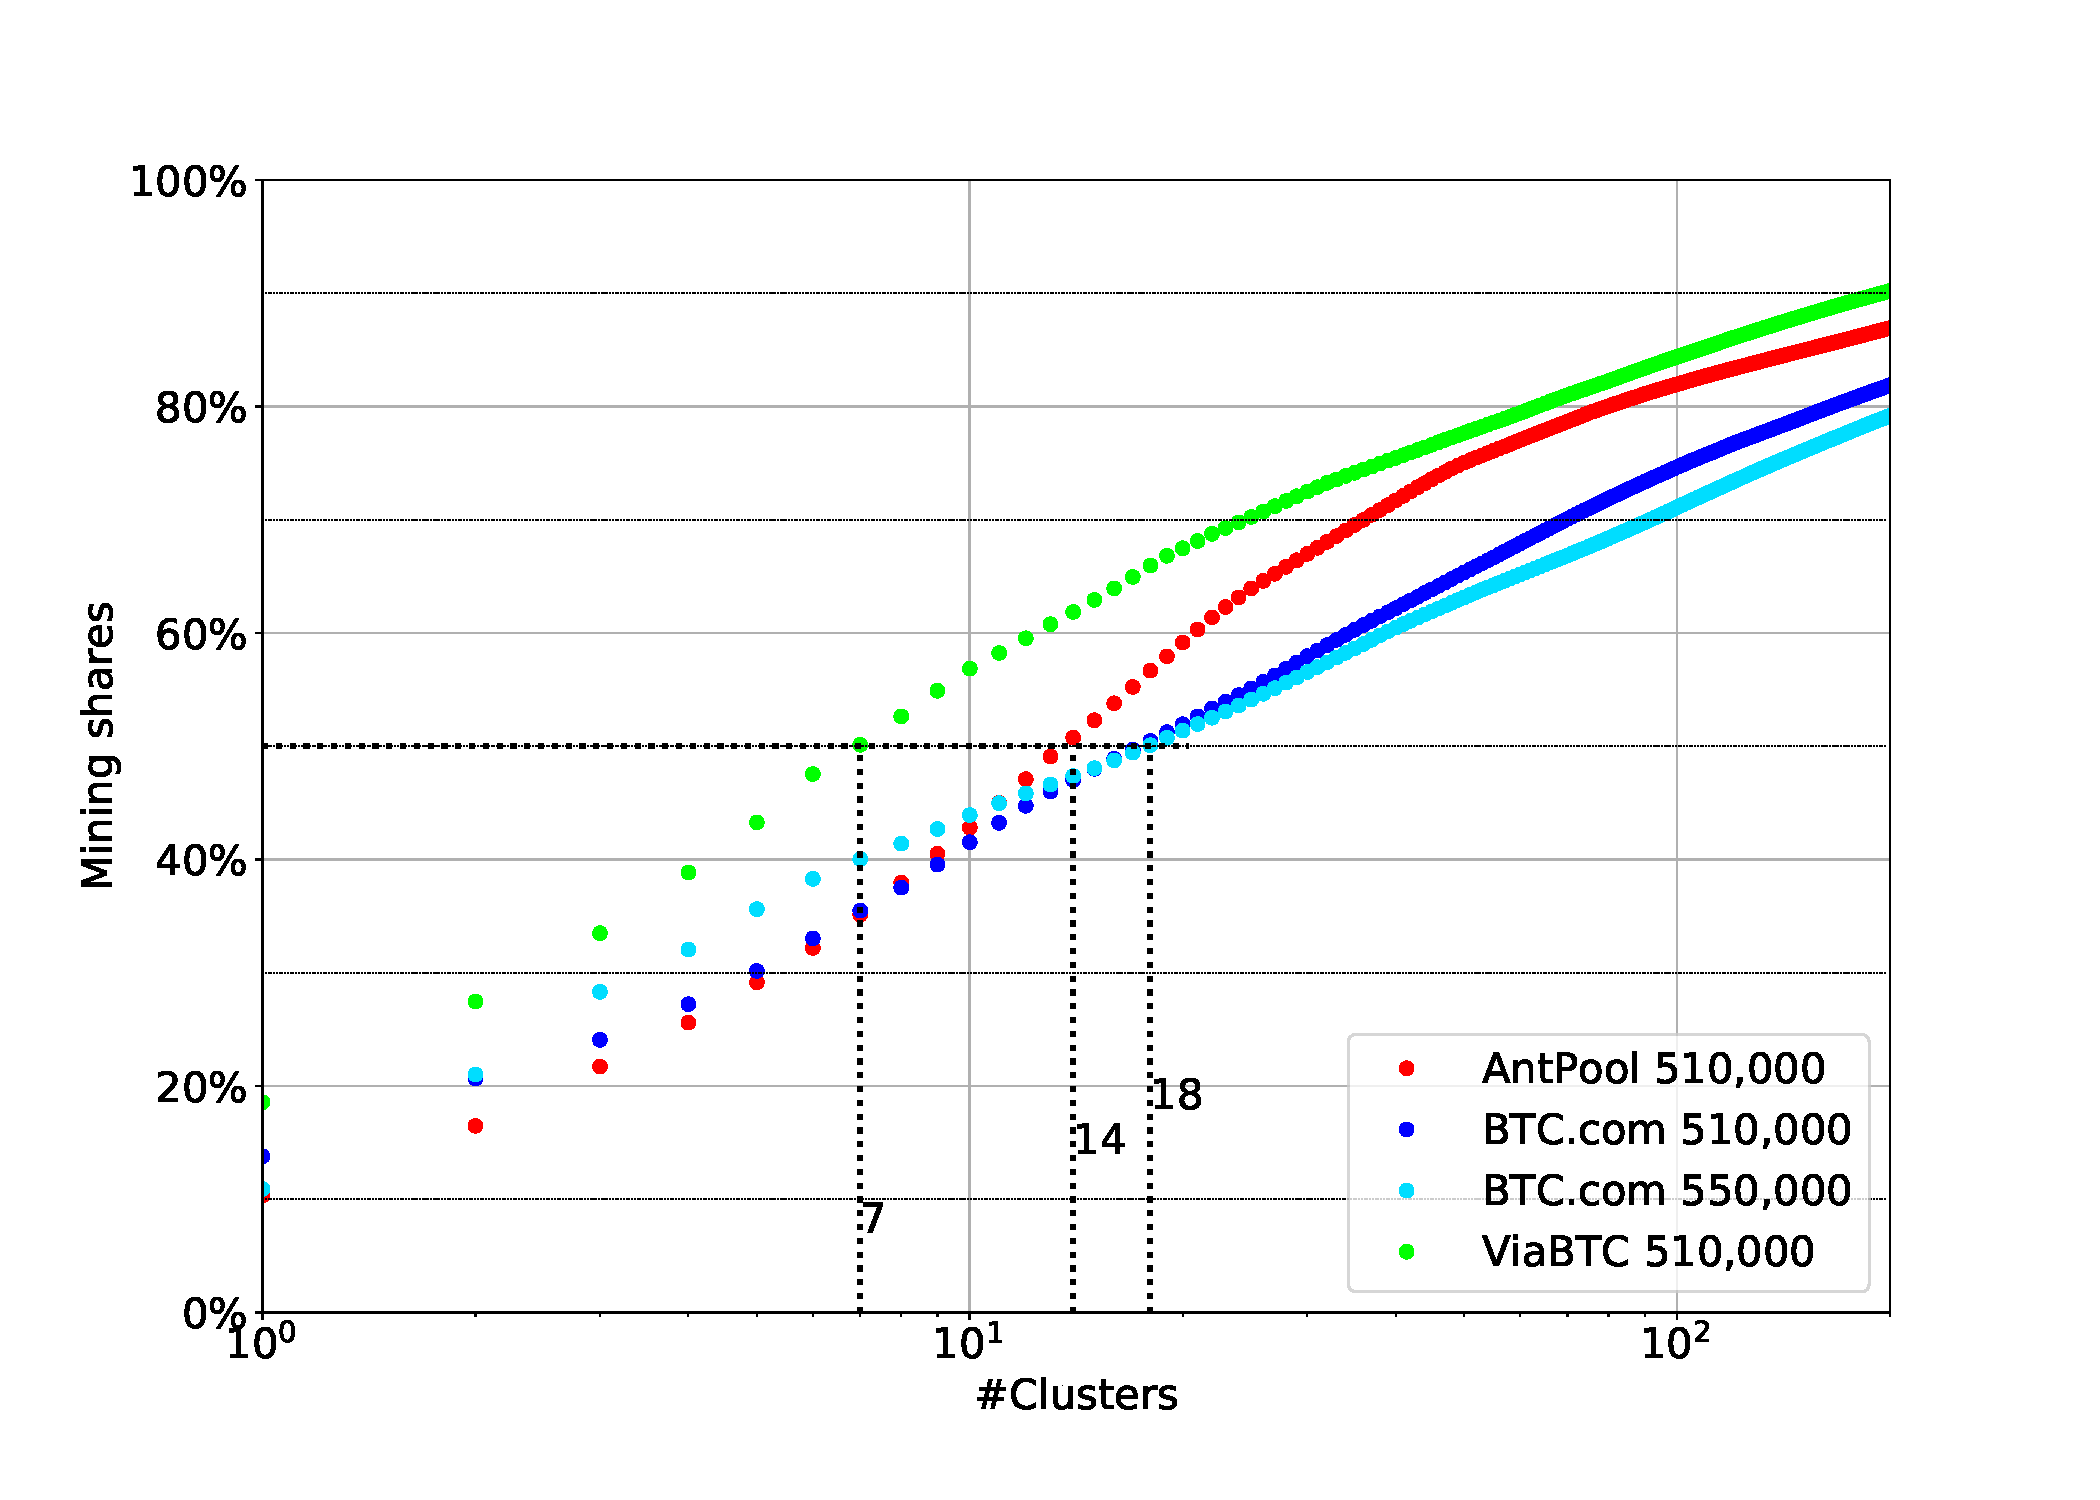
\includegraphics[width=0.8\textwidth]{images/pool_centralization.pdf}
        \\Cumulative sum of mining shares over clusters for each pool
    \end{figure}
\end{frame}

% \begin{frame}[fragile]{Pools Members | Cross-Pool Mining}
%     \setlength{\tabcolsep}{3pt}
%     \begin{table}
%         Cross-pool mining between block 510,000 and 514,032
%         \scalebox{.95}{
%             \begin{tabular}{@{}llllll@{}}
%             \toprule
%             Pool 1  & Pool 2  & \begin{tabular}[c]{@{}l@{}}Addresses \\ in common\end{tabular} & \begin{tabular}[c]{@{}l@{}}Clusters \\ in common\end{tabular} & \begin{tabular}[c]{@{}l@{}}BTC from\\ Pool 1\end{tabular} & \begin{tabular}[c]{@{}l@{}}BTC from\\ Pool 2\end{tabular} \\ \midrule
%             BTC.com & AntPool & 537 (1.58\%) & 434 (3.2\%)        & 664.3 (5.5\%)                                               & 176.8 (7.6\%)                                                \\
%             AntPool & ViaBTC  & 115 (0.54\%) & 196  (2.4\%)      & 11.1  (0.47\%)                                               & 102.6 (2.4\%)                                                \\
%             ViaBTC  & BTC.com & 250 (0.91\%)  & 267  (2.3\%)     & 175.4 (4.1\%)                                               & 174.1 (1.4\%)                                               \\ \bottomrule
%             \end{tabular}
%         }
%     \end{table}
% \end{frame}

\begin{frame}[fragile]{Pools Members | Cross-Pool Mining}
    \begin{figure}
        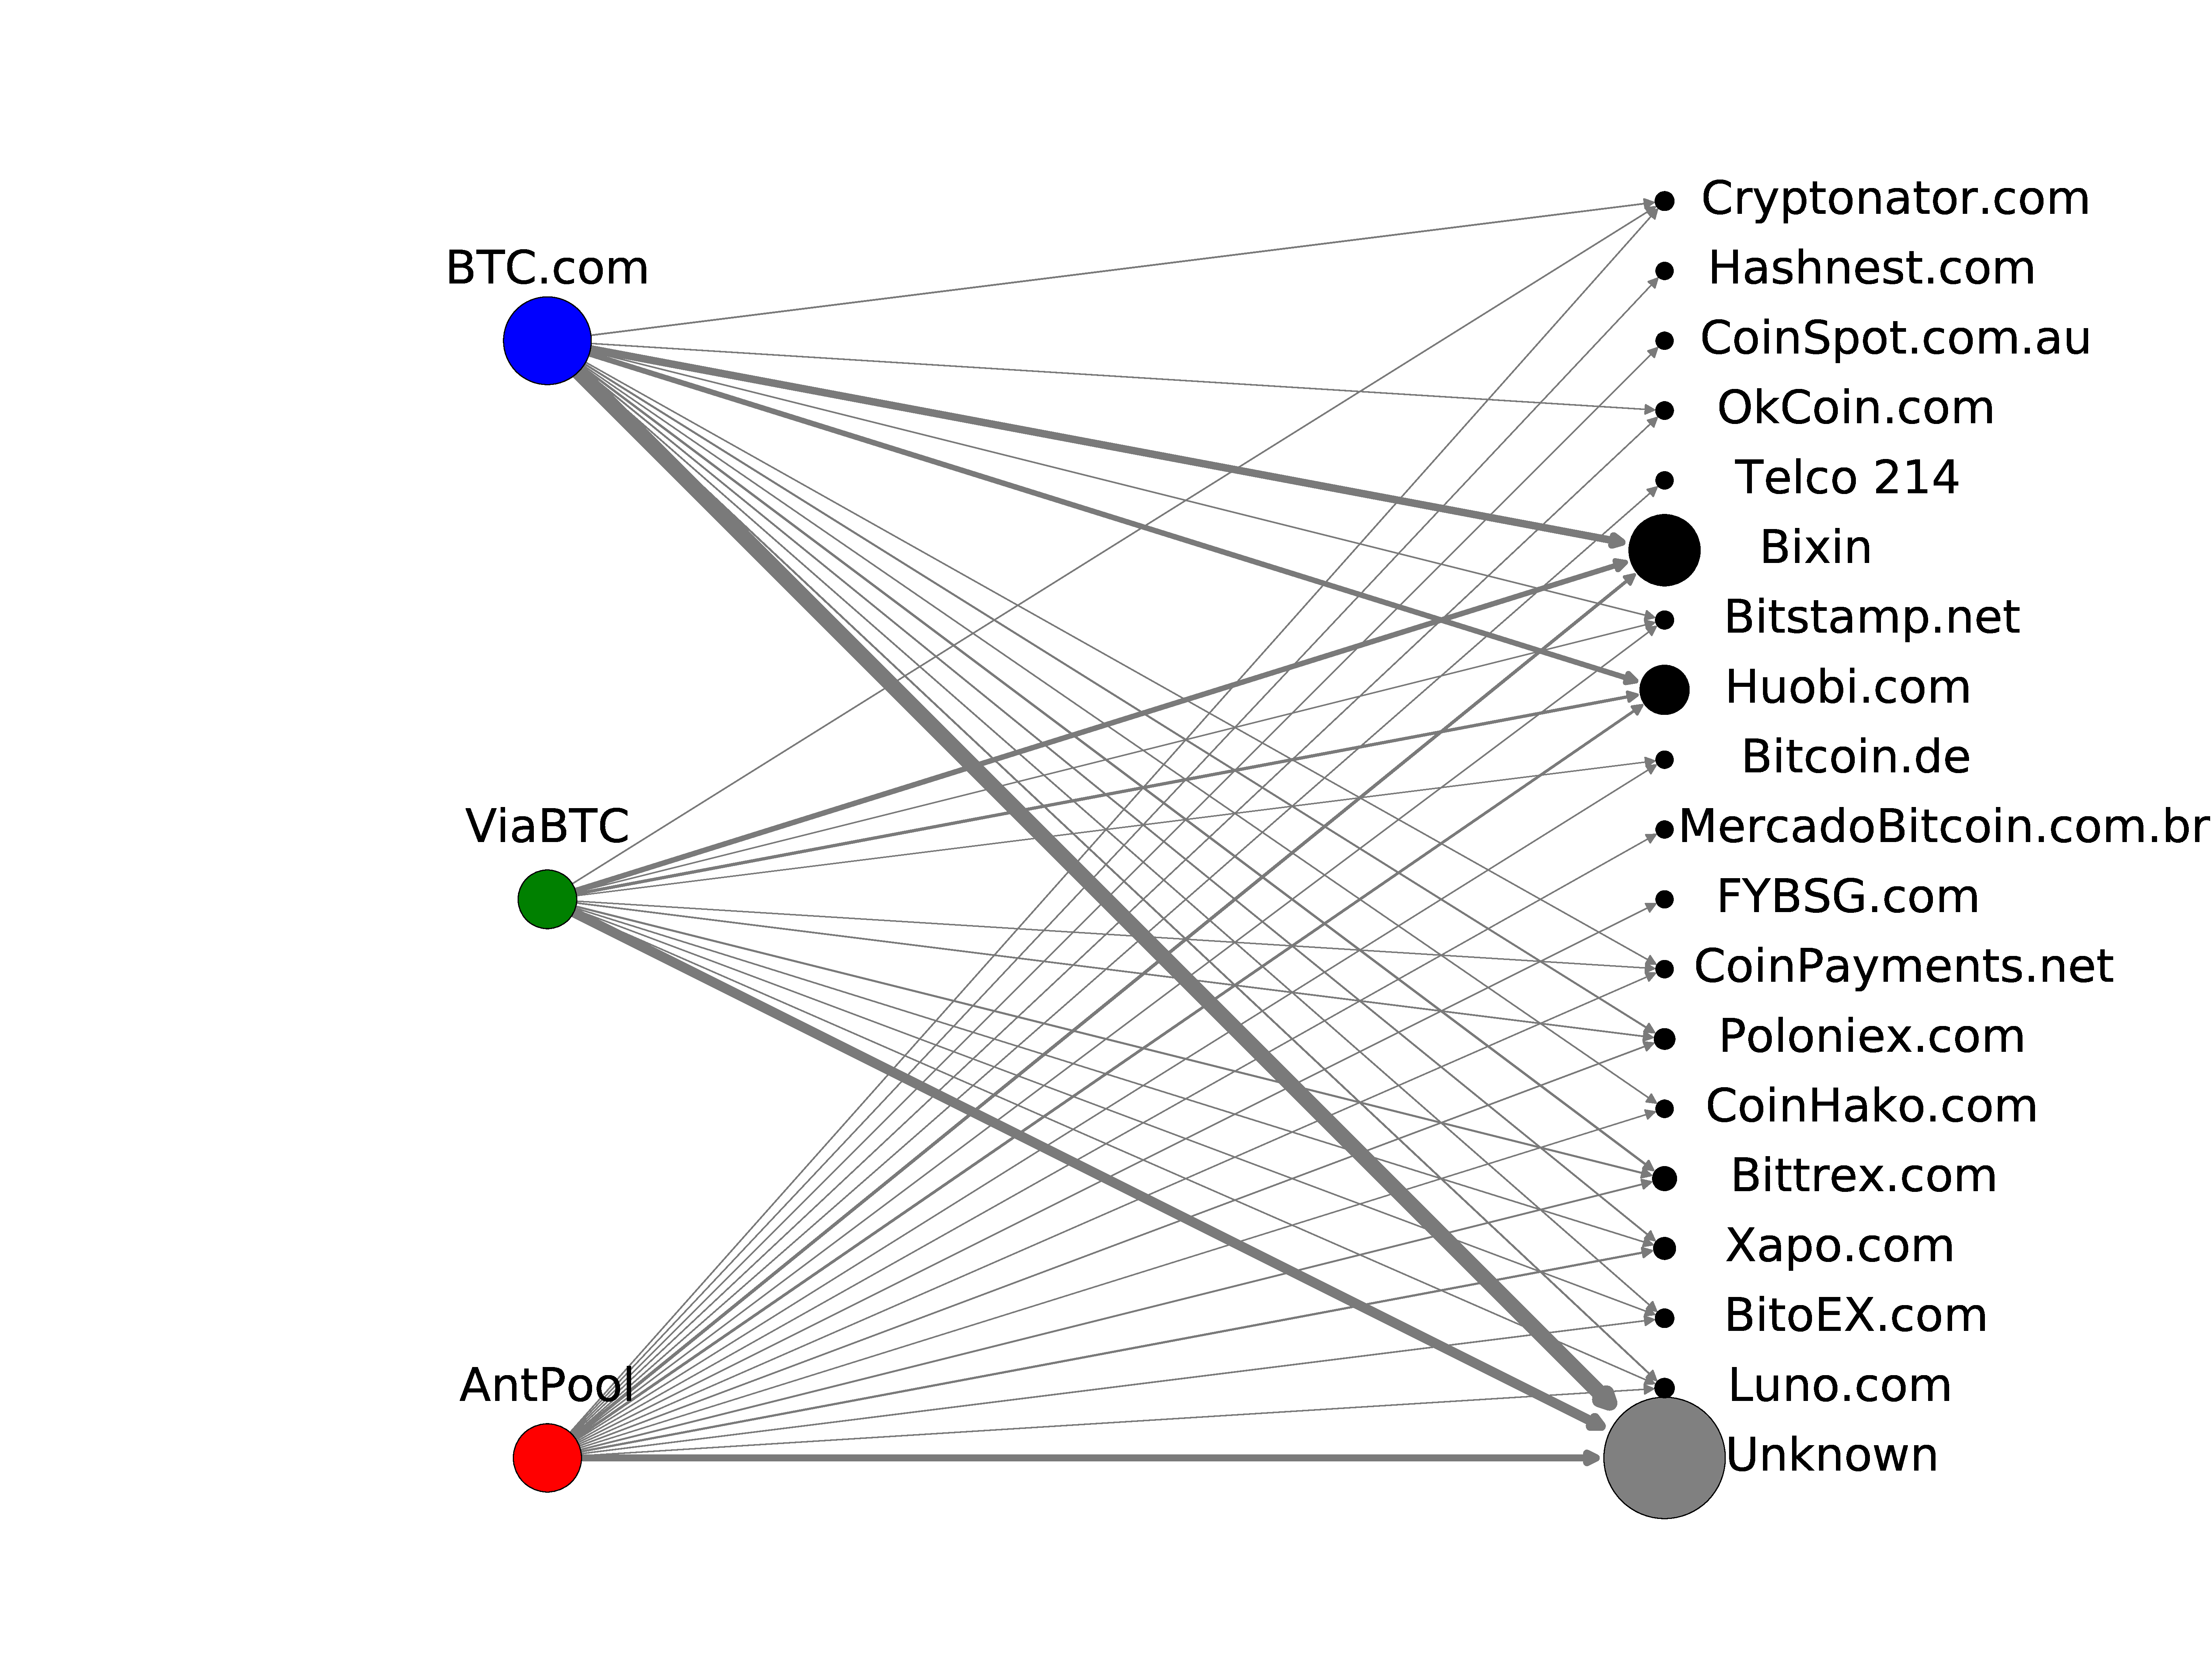
\includegraphics[width=0.8\columnwidth]{images/payments_graph_400.pdf}
        \\Distribution of mining rewards among top members
    \end{figure}
\end{frame}


\begin{frame}[fragile]{Pools Members | Main Entities}
    \setlength{\tabcolsep}{2pt}
    \begin{table}
        Cross-pool mining between block 510,000 and 514,032. W: wallet provider, E: exchange service, P: mining pool, M: unknown mining entity
        \scalebox{0.65}{
            \begin{tabular}{@{}llrrrrrrrrrr@{}}
            \toprule
                          &  & \multicolumn{3}{c}{BTC.com}   & \multicolumn{3}{c}{AntPool}   & \multicolumn{3}{c}{ViaBTC}    &  \\ \cmidrule(lr){3-5} \cmidrule(lr){6-8} \cmidrule(lr){9-11}
            Entity/Actor             & Service        & BTC     & \%BTC & \#Addr. & BTC     & \%BTC & \#Addr. & BTC     & \%BTC & \#Addr. & Total BTC \\ \midrule
            Unknown             & ?       & 8930.39 & \textbf{\textcolor{red}{74.07}} & 13286       & 1682.25 & \textbf{\textcolor{red}{72.09}} & 8888        & 2877.02 & \textbf{\textcolor{red}{67.17}} & 4845        & 13489.67  \\ 
            Bixin               & W+E+P   & 1663.75 & 13.80 & 1061        & 241.28  & 10.34 & 546         & 795.36  & 18.57 & 476         & 2700.39   \\ 
            Huobi.com         & E       & 808.64  & 6.71  & 964         & 142.04  & 6.09  & 759         & 225.50  & 5.27  & 322         & 1176.19   \\ 
            % Old mining clusters & M       & 426.72  & 3.54  & 3793        & 141.84  & 6.08  & 3081        & 300.62  & 7.02  & 1033        & 869.19    \\ 
            Bittrex.com         & E       & 83.71   & 0.69  & 348         & 29.56   & 1.27  & 251         & 43.36   & 1.01  & 177         & 156.63    \\ 
            Xapo.com            & W       & 26.96   & 0.22  & 94          & 70.75   & 3.03  & 64          & 5.79    & 0.14  & 33          & 103.50    \\ 
            Poloniex.com        & E       & 42.65   & 0.35  & 381         & 11.52   & 0.49  & 268         & 19.97   & 0.47  & 139         & 74.15     \\ 
            Luno.com            & W+E     & 36.59   & 0.30  & 258         & 4.06    & 0.17  & 104         & 4.39    & 0.10  & 60          & 45.04     \\ 
            Bitstamp.net        & E       & 8.94    & 0.07  & 57          & 3.55    & 0.15  & 38          & 3.91    & 0.09  & 22          & 16.39     \\ 
            Cryptonator.com     & W+E     & 5.75    & 0.05  & 80          & 0.70    & 0.03  & 41          & 2.70    & 0.06  & 33          & 9.15      \\ 
            % BitoEX.com          & W       & 5.09    & 0.04  & 23          & 1.12    & 0.05  & 35          & 2.19    & 0.05  & 4           & 8.39      \\ 
            % CoinHako.com        & W+E     & 3.59    & 0.03  & 4           & 0.29    & 0.01  & 3           & 0.24    & 0.01  & 2           & 4.12      \\ 
            % Bitcoin.de          & E       & 1.86    & 0.02  & 26          & 0.76    & 0.03  & 13          & 0.58    & 0.01  & 7           & 3.19      \\ 
            \bottomrule
            \end{tabular}
        }
    \end{table} 
\end{frame}

\section{Conclusion} 
\begin{frame}[fragile]{Conclusion}
    \begin{enumerate}
        \item Mining centralization follows a cyclical pattern
        \item Few companies and few countries lead the mining industry 
        \item Pools follow payout patterns
        \item Pools are centralized
        \item The majority of the pool members remain unknown
    \end{enumerate}
\end{frame}

\section{Future work} 
\begin{frame}[fragile]{Future work}
    \begin{itemize}
        \item Classification/characterization of entities 
        \item Collaborative tag sharing
        \item Improve heuristics to get payout patterns
        \item Extend analysis to other pools
        \item IP-network traffic measurement
    \end{itemize}
\end{frame}
 
\begin{frame}[fragile]{Links}
    \begin{itemize}
        \item \textbf{Slides}:\\ \url{https://github.com/MatteoRomiti/WEIS_Deep_Dive_slides} 
        \item \textbf{Graphsense}:\\ \url{https://graphsense.info/} 
        \item \textbf{Code}:\\ \url{https://github.com/MatteoRomiti/Deep_Dive_BTC_Mining_Pools} 
        \item \textbf{Data}:\\ \url{https://zenodo.org/}
    \end{itemize}
\end{frame}


% \begin{frame}[allowframebreaks]{References}
%   \bibliography{demo}
%   \bibliographystyle{abbrv}
% \end{frame}

\section{Appendix}
\begin{frame}[fragile]{Block Attribution | Results}
    \begin{figure}
        \centering
        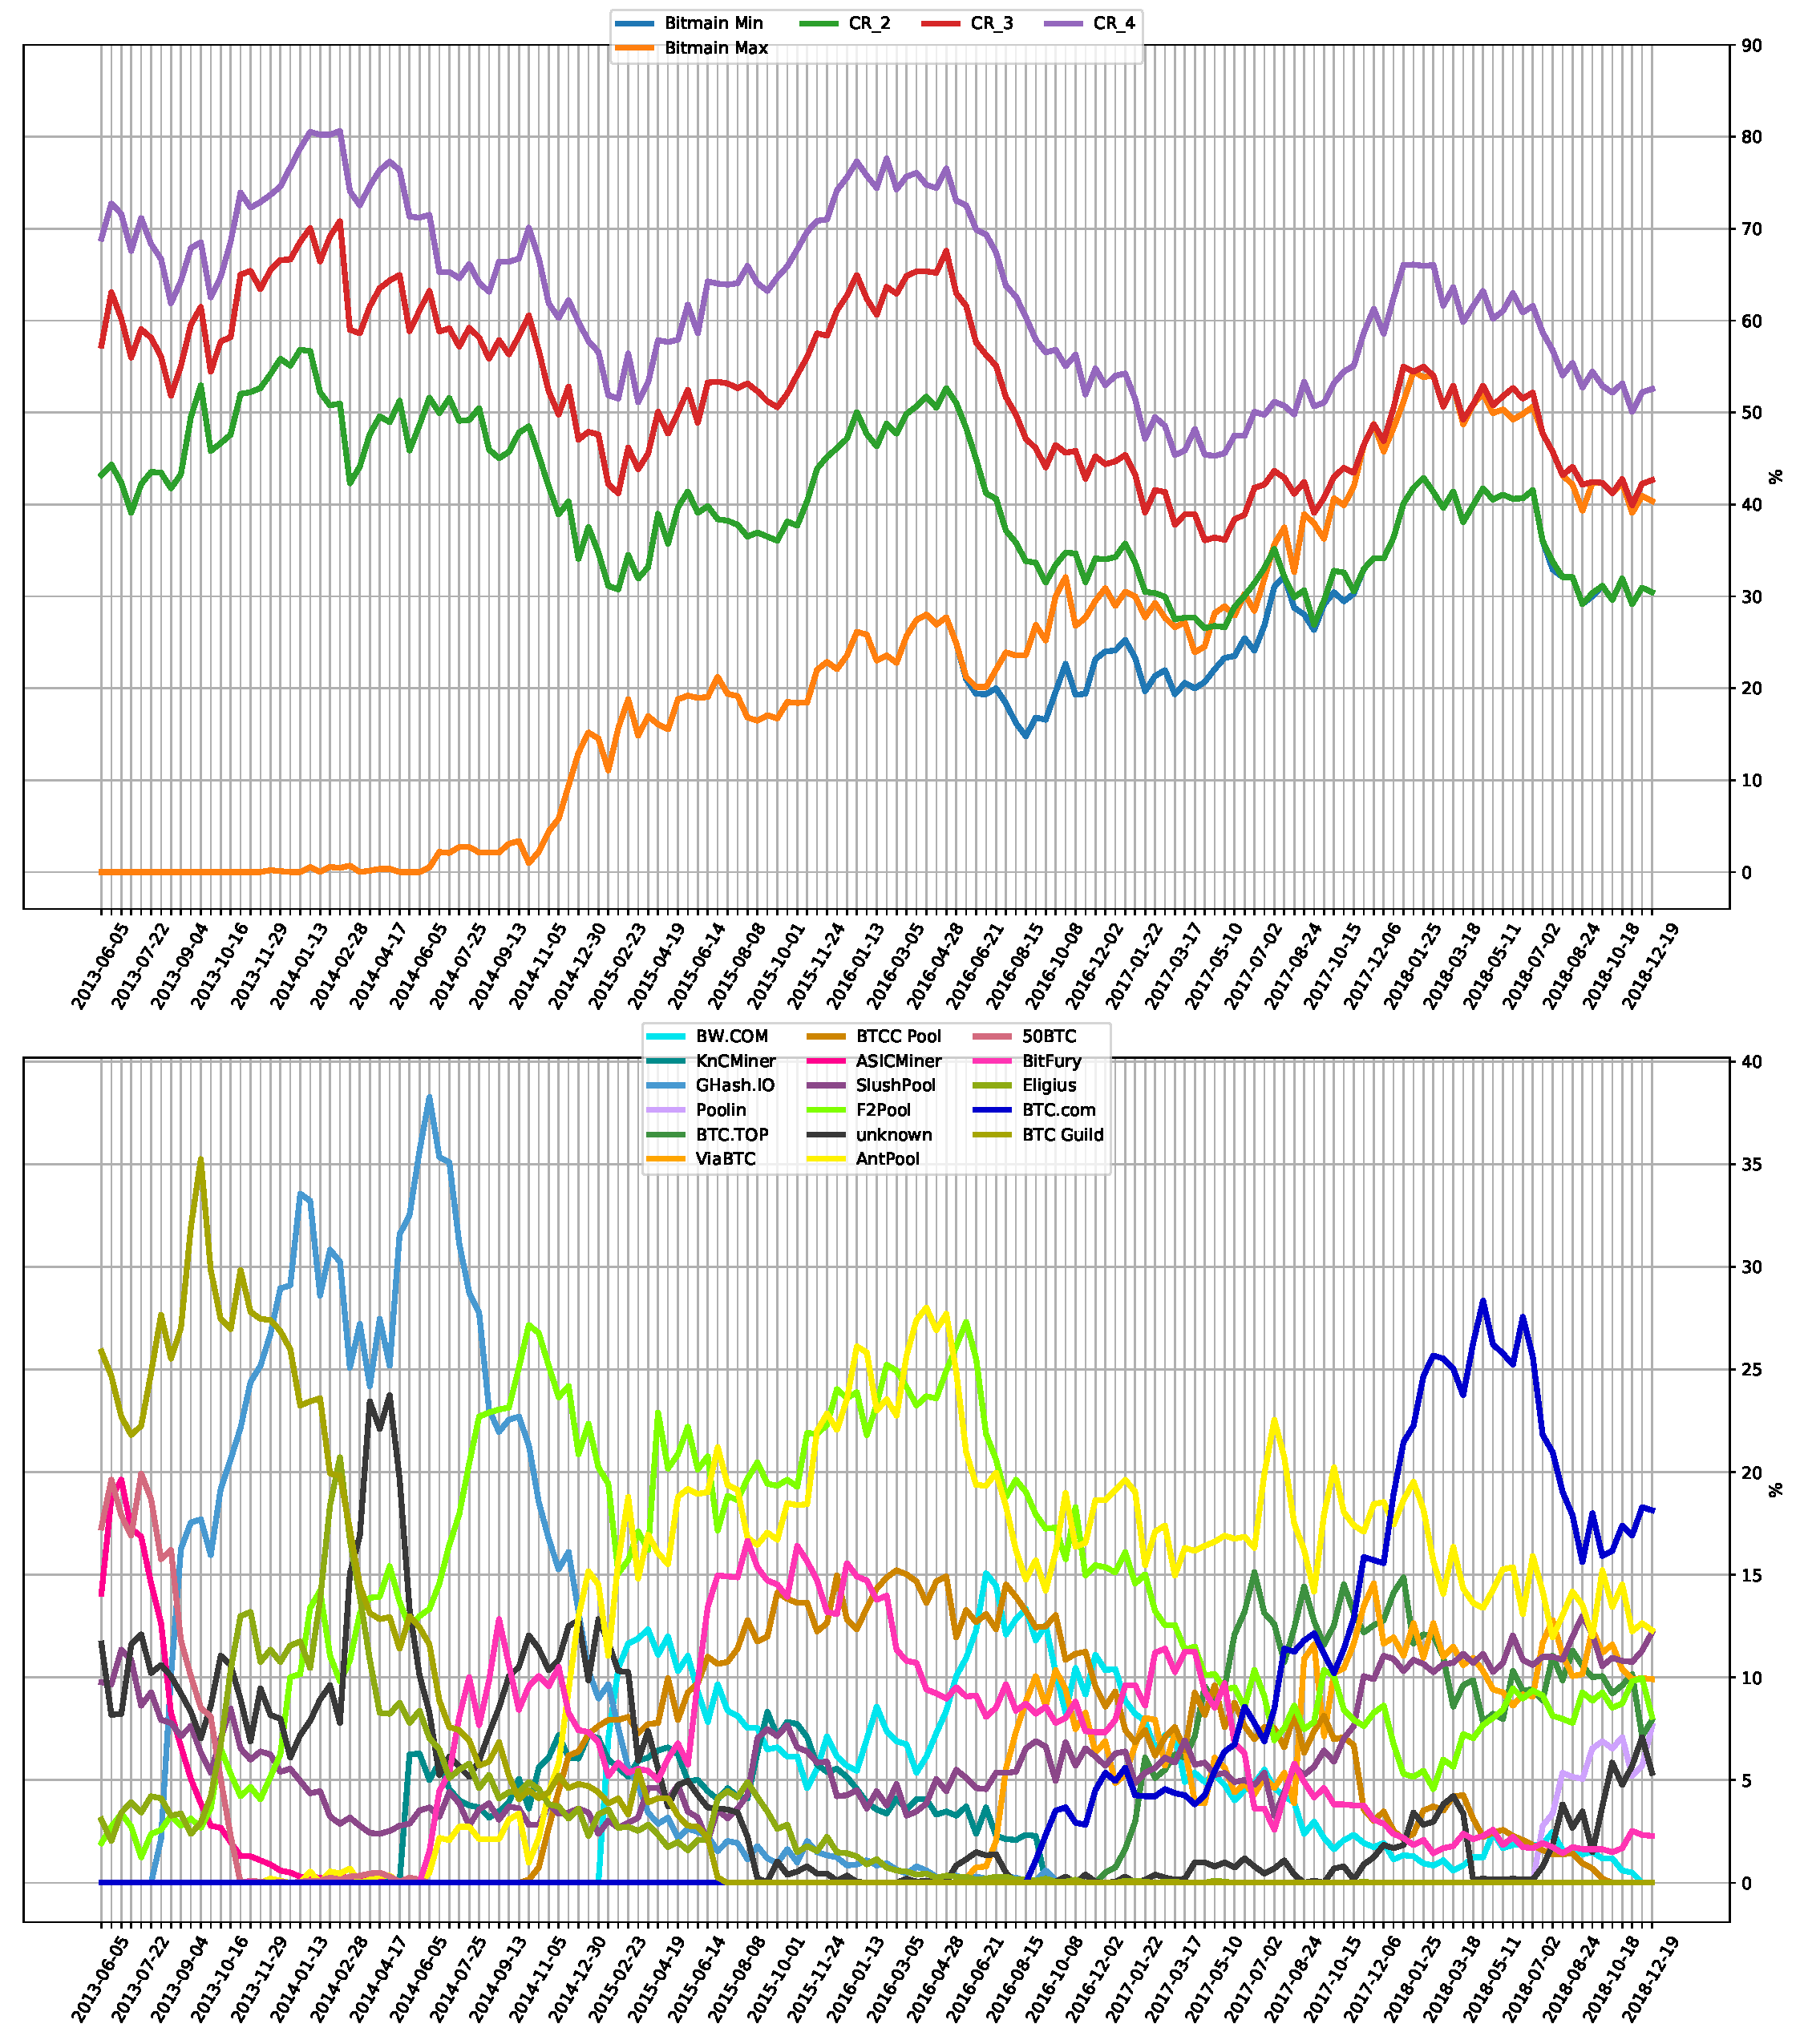
\includegraphics[width=.6\textwidth]{images/mining_distribution_157.pdf}
        \caption{Concentration indeces and mining shares.} \label{fig:mining_distribution}
    \end{figure}
\end{frame}


\begin{frame}[fragile]{Pools Members | Cross-Pool Unknown Mining}
    \begin{table}[]
        \caption{Cross-pool mining of the ten largest unknown mining clusters sorted by total amount of BTC received by the three pools in the time period between block 510,000 and 514,032 ($\sim$ 4 weeks).}\label{table:crosspool_unknown_entities}

        \scalebox{0.8}{
            \begin{tabular}{@{}rrrrrrrrr@{}}
            \toprule
                       & \multicolumn{2}{c}{BTC.com}                         & \multicolumn{2}{c}{AntPool}                         & \multicolumn{2}{c}{ViaBTC}                          &                      &             \\ \cmidrule(lr){2-3} \cmidrule(lr){4-5} \cmidrule(lr){6-7}
            Cluster ID & \multicolumn{1}{c}{BTC} & \multicolumn{1}{c}{\%BTC} & \multicolumn{1}{c}{BTC} & \multicolumn{1}{c}{\%BTC} & \multicolumn{1}{c}{BTC} & \multicolumn{1}{c}{\%BTC} & \multicolumn{1}{c}{\begin{tabular}[c]{@{}c@{}}Mined\\BTC\end{tabular}} & \multicolumn{1}{c}{\begin{tabular}[c]{@{}c@{}}Total BTC\\Received\end{tabular}}     \\ \midrule
            327539880  & 409.34                  & 3.40                      & 122.10                  & 5.23                      & 258.55                  & 6.04                      & 789.99               & 521,939  \\
            324067473  & 295.02                  & 2.45                      & 90.44                   & 3.88                      & 189.15                  & 4.42                      & 574.61               & 3,756,583  \\
            350822682  & 244.77                  & 2.03                      & 9.29                    & 0.40                      & 182.92                  & 4.27                      & 436.98               & 110,566 \\
            350824718  & 244.67                  & 2.03                      & 65.65                   & 2.81                      & 46.20                   & 1.08                      & 356.52               & 112,680 \\
            333653856  & 153.02                  & 1.27                      & 54.02                   & 2.31                      & 83.60                   & 1.95                      & 290.63               & 130,680   \\
            372448840  & 181.10                  & 1.50                      & 33.64                   & 1.44                      & 55.73                   & 1.30                      & 270.48               & 882,713  \\
            234254928  & 93.31                   & 0.77                      & 27.18                   & 1.16                      & 58.68                   & 1.37                      & 179.17               & 905,101   \\
            249123673  & 15.63                   & 0.13                      & 0.40                    & 0.02                      & 107.23                  & 2.50                      & 123.26               & 6,812,938 \\
            349962609  & 8.67                    & 0.07                      & 39.01                   & 1.67                      & 19.74                   & 0.46                      & 67.41                & 1,173,892 \\
            311503667  & 38.94                   & 0.32                      & 7.47                    & 0.32                      & 7.77                    & 0.18                      & 54.18                & 486,338 \\
            \bottomrule
            \end{tabular}
        }
    \end{table}
\end{frame}

\begin{frame}[fragile]{Payout Patterns | Methodology}
    \begin{algorithm}[H]
        \caption{Find payout patterns in BTC.com, AntPool and ViaBTC.}\label{algo:blocks_addresses}
        \begin{algorithmic}[1]
            \For{each pool}
                \For{each mined block}
                    \State get coinbase flow of block
                    \State compute number of addresses at each step of the coinbase flow
                    \State save results
                \EndFor
                \State plot data and look for common patterns among flows
            \EndFor
        \end{algorithmic}
    \end{algorithm}
\end{frame}

\begin{frame}[fragile]{Payout Patterns | Methodology}
    \begin{figure}
        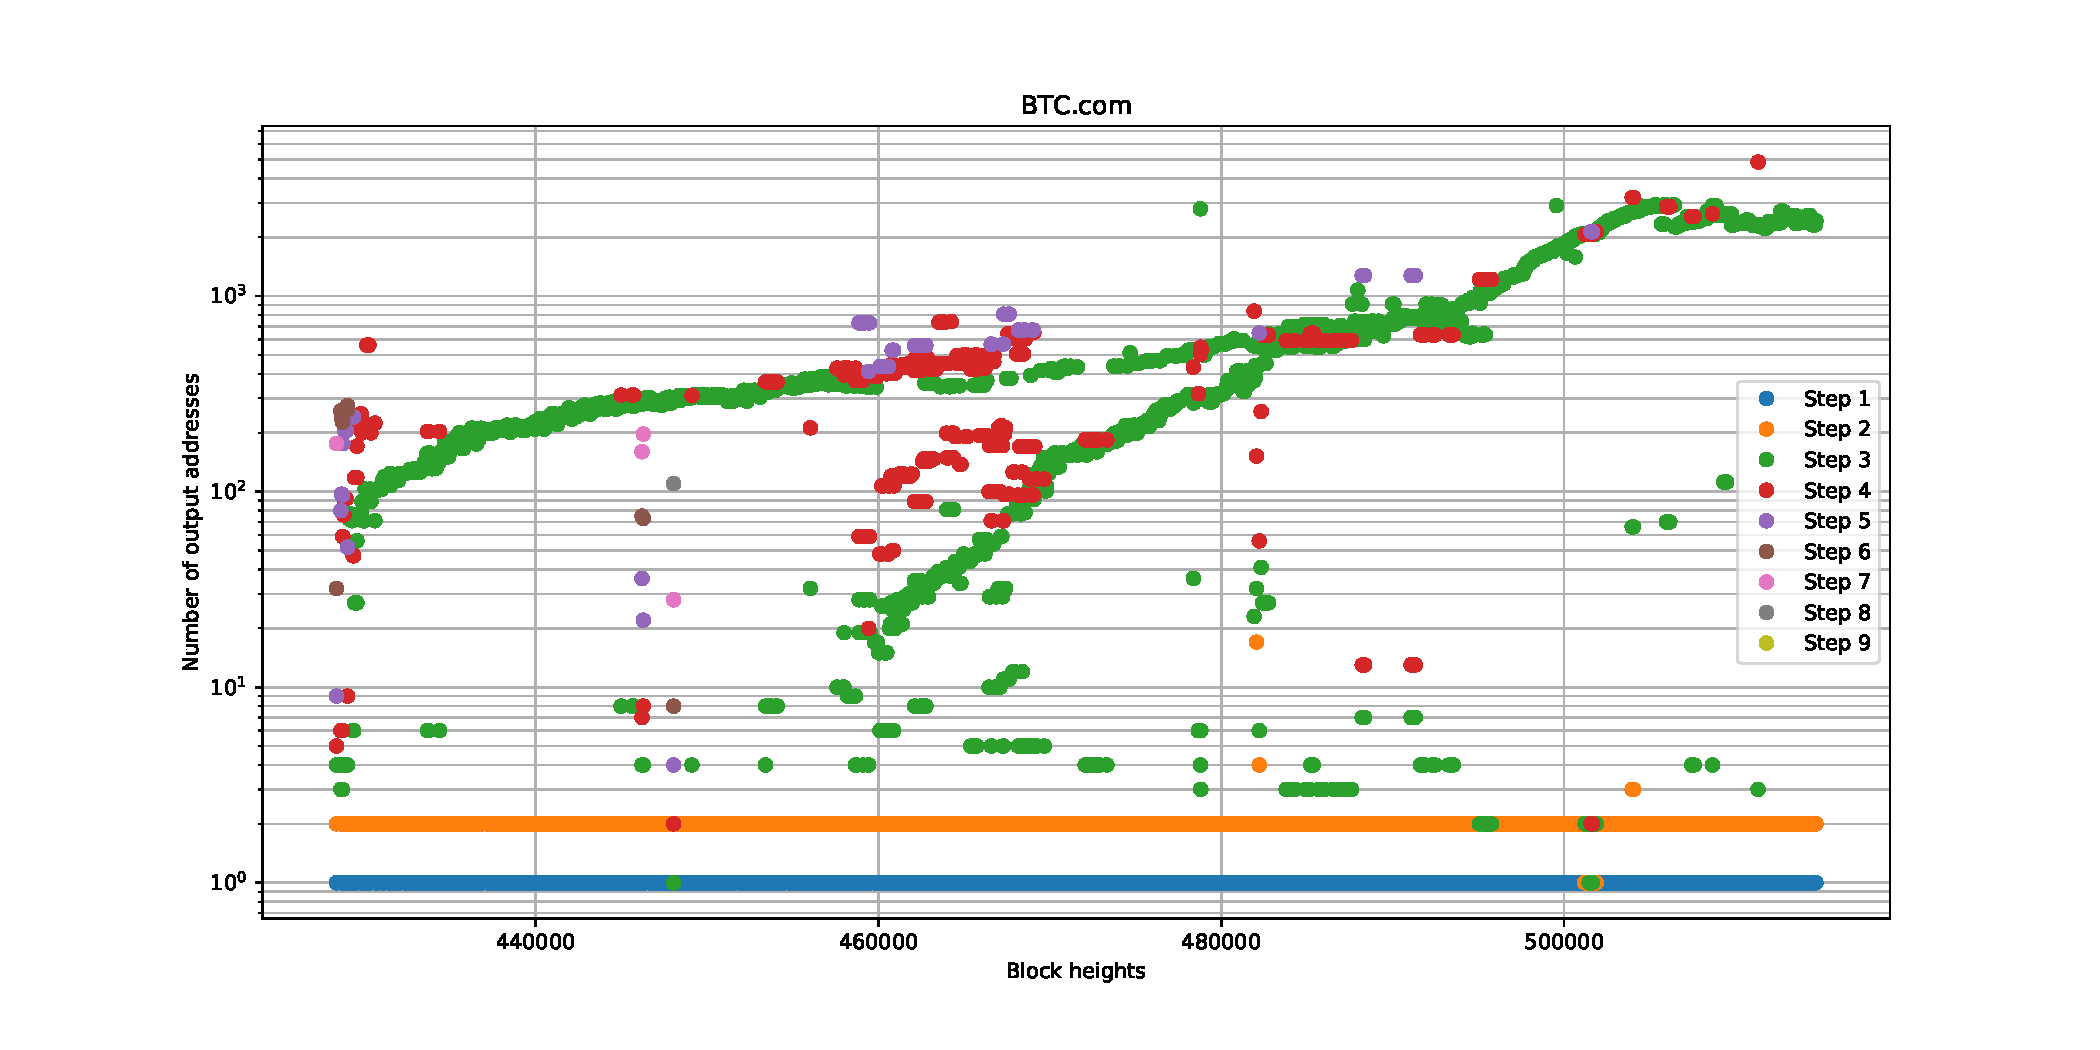
\includegraphics[width=\textwidth]{images/payout_trend_BTC_com.pdf}
        \caption{Payout trend for BTC.com} \label{fig:payout_trend_BTCcom}
    \end{figure}
\end{frame}

% \begin{frame}[fragile]{Appendix}
% % number of addresses per step 
%     \begin{figure}
%         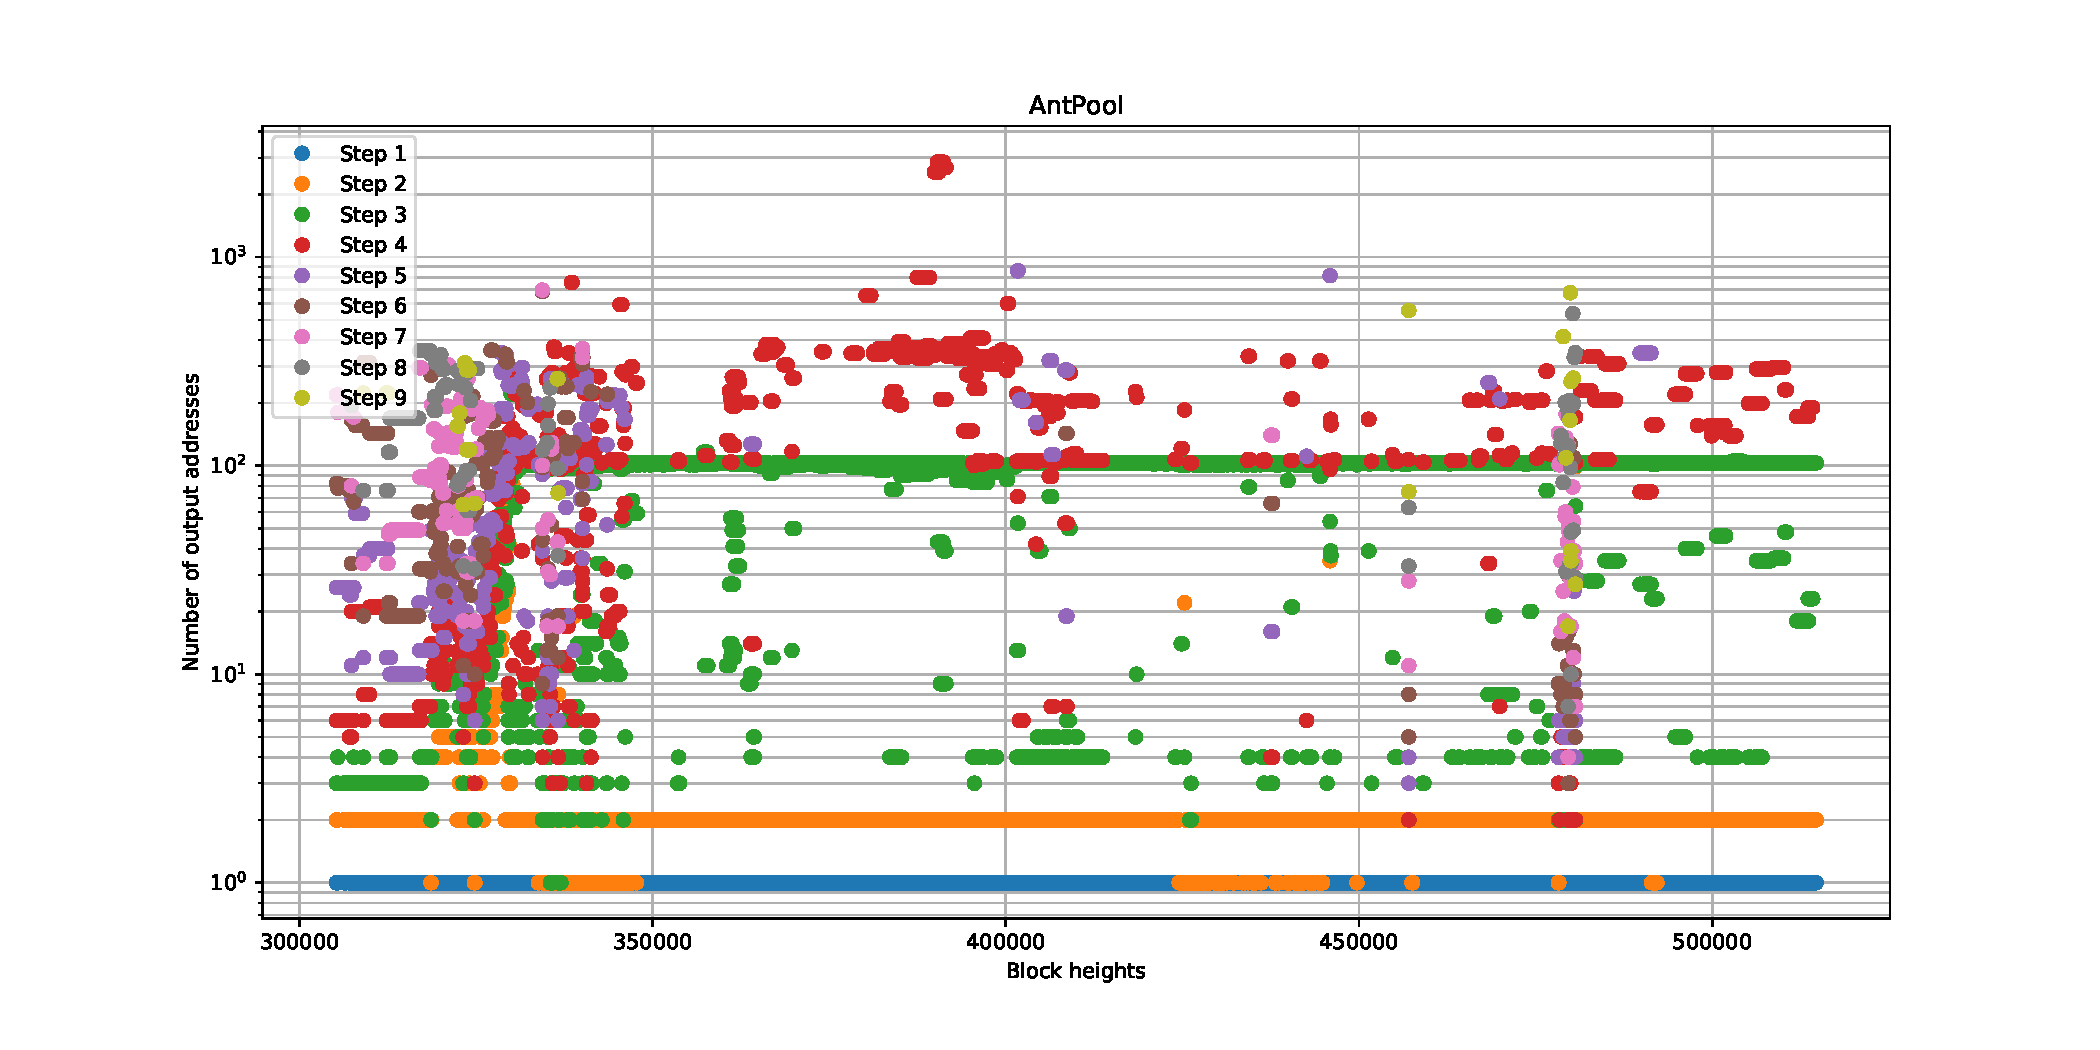
\includegraphics[width=0.8\textwidth]{images/payout_trend_AntPool.pdf}
%         \caption{Payout trend for AntPool} \label{fig:payout_trend_AntPool}
%     \end{figure}
% \end{frame}

% \begin{frame}[fragile]{Appendix}
% % number of addresses per step 
%     \begin{figure}
%         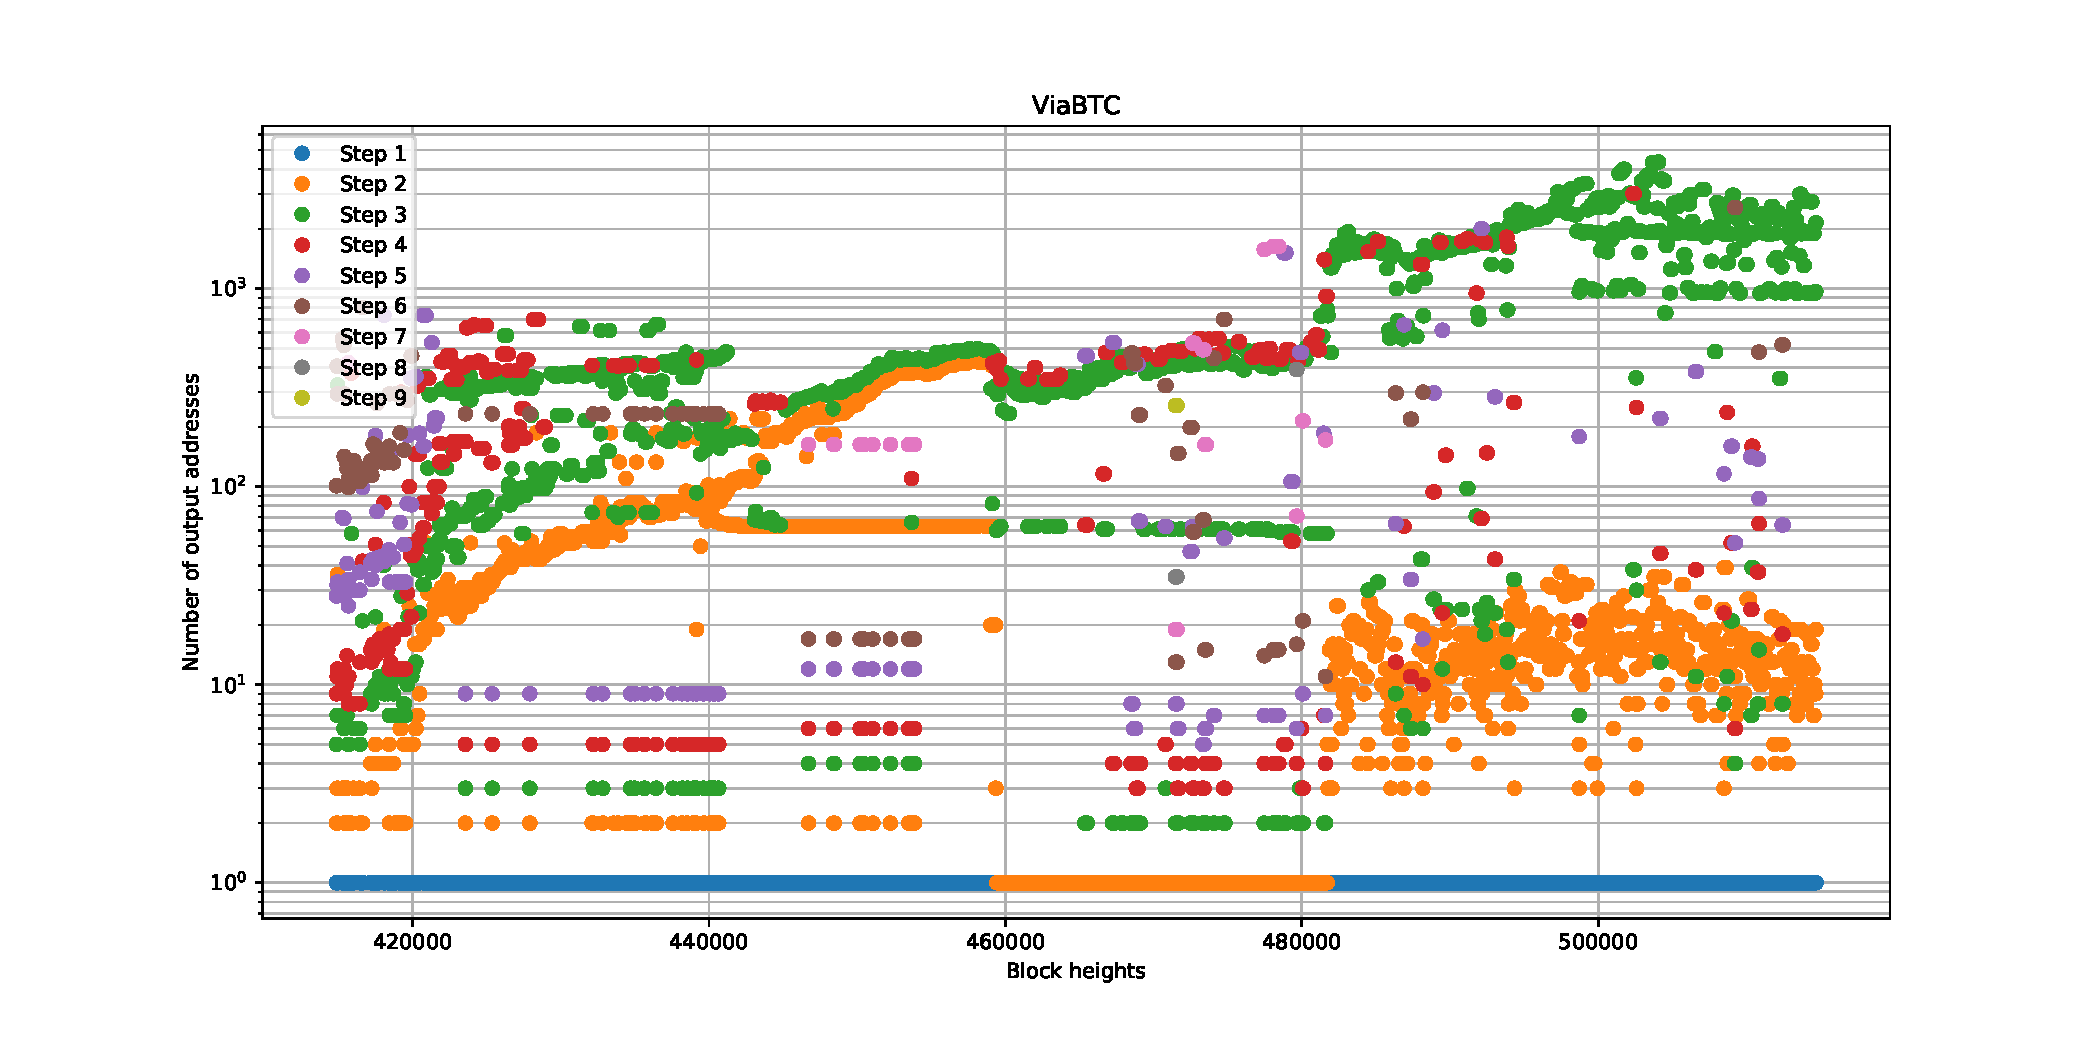
\includegraphics[width=0.8\textwidth]{images/payout_trend_ViaBTC.pdf}
%         \caption{Payout trend for ViaBTC} \label{fig:payout_trend_ViaBTC}
%     \end{figure}
% \end{frame}


\end{document}
